\documentclass[a4paper,12pt]{article}
\usepackage[utf8]{inputenc}
\usepackage[slovak]{babel}
\usepackage{hyperref}
\usepackage{graphicx}
\usepackage{fancyhdr}
\usepackage{titlesec}
\usepackage{float}

% Nastavenie titulnej strany
\begin{document}

\begin{titlepage}
    \centering
    \vspace*{1cm}
    \Large{\textbf{Technická univerzita v Košiciach}\\
    Fakulta elektrotechniky a informatiky}\\
    \vfill
    \large{Formálne jazyky}\\
    \large{Dokumentácia k obhajobe zadania}
    \vfill
    \begin{flushleft}
        Lukáš Čeč\\
        Akademický rok: 2024/2025\\
        Študijný program: Informatika
    \end{flushleft}
\end{titlepage}

\tableofcontents
\newpage

\section{Formulácia zadania}

Cieľom zadania je implementovať jednoduchý generátor konečnostavových automatov (NKA) zo zadaného regulárneho výrazu využitím metódy jeho syntaktickej analýzy zhora nadol rekurzívnym zostupom. Pri vypracovaní zadania nie je povolené použitie žiadneho existujúceho generátora jazykových procesorov.

\section{Vypracovanie zadania}

\subsection{Opis architektúry riešenia}

Navrhnuté riešenie je rozdelené na backendovú a frontendovú časť. Backend je implementovaný v jazyku Python pomocou frameworku FastAPI. Jeho úlohou je prijímať regulárny výraz vo forme reťazca, parsovať ho pomocou rekurzívne zostupného syntaktického analyzátora, generovať derivančný strom a následne zo stromu vytvárať nedeterministický konečný automat (NKA). Výsledný automat je možné testovať na vstupe.

Frontend je implementovaný v Next.js. Slúži na vizualizáciu derivačného stromu a interaktívne zadávanie regulárnych výrazov. Používateľ môže vkladať výrazy, zobraziť ich derivančné stromy a skúšať, či konkrétne slová daný automat akceptuje. Súčasťou rozhrania je aj história zadaných výrazov.

Komunikácia medzi frontendom a backendom prebieha cez REST API. Každý regulárny výraz je na server odoslaný pomocou HTTP POST požiadavky, pričom odpoveď obsahuje serializovaný derivačný strom alebo výsledok simulácie automatu.

Celé riešenie je kontajnerizované pomocou Dockeru, aby bolo jednoducho spustiteľné na akomkoľvek systéme.

\subsection{Gramatika jazyka regulárnych výrazov (EBNF)}

Použitá gramatika jazyka regulárnych výrazov je nasledovná (v EBNF):

\begin{verbatim}
<regular>     ::= <alternative>

<alternative> ::= <sequence> { "|" <sequence> }

<sequence>    ::= { <element> }

<element>     ::= "{" <regular> "}"      // Iterácia (Kleeneho hviezda)
               |  "[" <regular> "]"      // Voliteľnosť (alebo eps)
               |  <symbol>
               |  "eps"                    // Epsilon

<symbol>      ::= znak okrem špeciálnych znakov {, }, [, ], |

\end{verbatim}

Vysvetlenie:
\begin{itemize}
    \item \textbf{Tranzitívny uzáver} \{\} označujú iteráciu (Kleeneho hviezda, t.j. ľubovoľne veľa opakovaní).
    \item \textbf{Voliteľnosť} [ ] označujú voliteľnosť (t.j. výraz v zátvorkách alebo nič).
    \item \textbf{Alternatíva} \textbar{} (pipe) vyjadruje alternatívu (alebo).
    \item \textbf{Epsilon} značí prázdne slovo.
    \item \textbf{Symbol} je ľubovoľný znak okrem vyššie uvedených špeciálnych znakov.
\end{itemize}

\subsection{Podrobný postup implementácie}

Implementácia sa skladá z niekoľkých hlavných častí:

\begin{enumerate}
    \item \textbf{Lexer} – Tokenizuje vstupný reťazec regulárneho výrazu na sekvenciu tokenov (zátvorky, symboly, operátory).
    \item \textbf{Parser} – Implementuje rekurzívne zostupný syntaktický analyzátor podľa EBNF gramatiky. Výsledkom je derivačný strom, v ktorom uzly reprezentujú pravidlá gramatiky a listy konkrétne symboly.
    \item \textbf{Konštrukcia NKA} – Prechádza derivačný strom a podľa typu uzla (sekvencia, alternatíva, iterácia, voliteľnosť) generuje príslušnú štruktúru NKA pomocou známych konštrukčných pravidiel (napr. Thompsonova konštrukcia).
    \item \textbf{Transofrmácia stromu} – Pre vizualizáciu na frontende sa strom transformuje do JSON formátu, kde každý uzol obsahuje svoj popis a deti.
    \item \textbf{Simulátor NKA} – Slúži na overenie, či dané slovo je akceptované vytvoreným automatom, využíva uzávierku epsilon-pravidiel.
    \item \textbf{Frontend vizualizácia} – Pomocou React Flow sa na základe JSON stromu vykreslí interaktívny graf derivačného stromu.
    \item \textbf{História výrazov a testovanie slov} – Frontend si udržiava históriu výrazov a umožňuje testovať slová na prijatie automatom.
    \item \textbf{Dockerizácia} – Backend aj frontend sú zabalené v separátnych Docker kontajneroch, spúšťané pomocou docker-compose.
\end{enumerate}

\subsection{Ukážka vstupu a prezentácia výsledkov}

\textbf{Príklad regulárneho výrazu:}
\begin{verbatim}
{a|b}[c]
\end{verbatim}

\textbf{Derivačný strom (vizuálne):}
\begin{figure}[H]
    \centering
    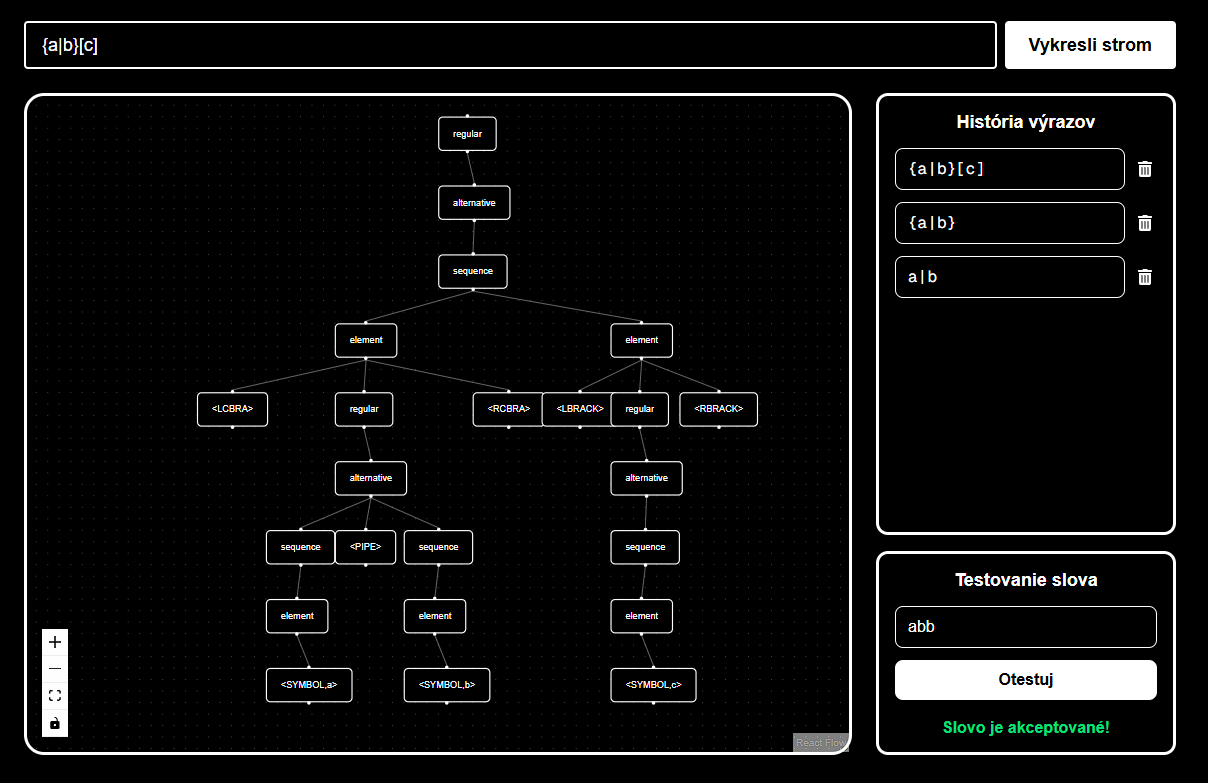
\includegraphics[width=1\linewidth]{tree.png}
    \caption{Ukážka derivačného stromu}
    \label{fig:tree}
\end{figure}


\textbf{Príklad simulácie:}

\begin{itemize}
    \item \texttt{regex = \{a|b\}[c]}, slovo \texttt{ab} $\rightarrow$ akceptované
    \item \texttt{regex = \{a|b\}[c]}, slovo \texttt{ac} $\rightarrow$ akceptované
    \item \texttt{regex = \{a|b\}[c]}, slovo \texttt{a} $\rightarrow$ akceptované
    \item \texttt{regex = \{a|b\}[c]}, slovo \texttt{abc} $\rightarrow$ akceptované
    \item \texttt{regex = \{a|b\}[c]}, slovo \texttt{bc} $\rightarrow$ akceptované
    \item \texttt{regex = \{a|b\}[c]}, slovo \texttt{b} $\rightarrow$ akceptované
    \item \texttt{regex = \{a|b\}[c]}, slovo \texttt{d} $\rightarrow$ neakceptované
\end{itemize}

Na obrázku je možné vidieť zobrazenie derivačného stromu pre konkrétny regulárny výraz. Používateľ môže ľubovoľne zadávať vlastné výrazy, vidieť ich stromy a testovať ľubovoľné slová.

\subsection{Problémy a ich riešenie}

Pri implementácii sa vyskytli nasledovné problémy:
\begin{itemize}
    \item \textbf{Správne parsovanie zátvoriek a operátorov}: Bolo potrebné detailne ošetriť, aby sa zátvorky správne párovali a výrazy ako \{ab|c\} boli správne rozpoznané a rozdelené.
    \item \textbf{Vizualizácia stromu}: Bolo potrebné riešiť rozmiestnenie uzlov tak, aby bol strom čitateľný aj pri väčších výrazoch.
  
  
\end{itemize}

Všetky tieto problémy boli postupne riešené ladením, dôsledným testovaním rôznych prípadov a prečítaním odporúčanej literatúry k téme.

\subsection{Hodnotenie zadania}

Zadanie hodnotím ako veľmi zaujímavé, pretože som mohol priamo aplikovať teoretické poznatky z formálnych jazykov, tým že som si zadanie obohatil o prepojenie backendu s frontendom a vizualizáciou odovzdávaných dát. Práca s Dockerom mi umožnila pripraviť riešenie jednoducho spustiteľné na ľubovoľnom systéme.


\section{Vyhodnotenie a záver}

V zadaní sa podarilo úspešne implementovať generátor NKA zo zadaného regulárneho výrazu pomocou rekurzívne zostupného analyzátora. Riešenie vďaka webovej vizualizácii umožňuje jednoduché testovanie rôznych výrazov a slov. Celý systém je dockerizovaný a pripravený na jednoduché nasadenie. Ako možnosť rozšírenia do budúcnosti vidím napríklad podporu deterministických automatov, generovanie minimalizovaných automatov, podporu ďalších operácií v regulárnych výrazoch, alebo export automatu do grafického formátu.

\vspace{1cm}
\noindent
\textbf{Priložené súbory:}\\
README.txt -- EBNF gramatika\\
Zdrojové kódy (backend, frontend)\\
Dockerfile, docker-compose.yml\\


\end{document}
